\documentclass{article}
\usepackage[utf8]{inputenc}
\usepackage[letterpaper, portrait, margin=1in]{geometry}
\usepackage{multicol}
\usepackage{amsmath}
\usepackage{amssymb}
\usepackage{enumerate}
\setlength\parindent{0pt}
\usepackage{enumerate}
\usepackage{graphicx}
\graphicspath{ {./images/} }
\usepackage{fancyhdr}
\usepackage{tcolorbox}
\hyphenchar\font=-1
\usepackage{tabularx}

\newcommand{\header}[1]{\begin{large}\noindent #1\end{large}\\\rule{\textwidth}{0.5pt}}
\newcommand{\gap}{\medskip\\}
\newcommand{\centertext}[1]{\begin{center}#1\end{center}}
\newcommand{\bfrac}[2]{\left(\frac{#1}{#2}\right)}
\newcommand{\formula}[3]{\begin{center} \begin{tcolorbox}[title = #2] $$#3$$\end{tcolorbox}\end{center}}
\newcommand{\where}{\hspace{0.5cm} \textrm{where} \hspace{0.5cm}}
\newcommand{\hgap}{\hspace{0.5cm}}
\newcommand{\pfrac}[2]{\frac{\partial #1}{\partial #2}}
\newcommand{\sheader}[1]{\underline{#1:}}
\newcommand{\doubleformula}[4]{\begin{center} \begin{tcolorbox}[title = #2] $$#3$$\\$$#4$$\end{tcolorbox}\end{center}}
\newcommand{\curly}[1]{\left\{#1\right\}}
\newcommand{\proj}[2]{{}\textrm{proj}_{#1}\left(#2\right)}

\newcommand{\ds}{\displaystyle}
\newcommand{\Arg}{\textrm{Arg}}

\newcommand{\tripleformula}[5]{\begin{center} \begin{tcolorbox}[title = #2] $$#3$$\\$$#4$$\\$$#5$$\end{tcolorbox}\end{center}}

\begin{document}
    \begin{center}
        \Large PHYS 304 Review Notes\\
        \normalsize Reese Critchlow
    \end{center}

    \header{General Forms for Solving Schrodinger Equations in Bound States}

    For a Schrodinger equation of the form:
    \begin{align*}
        -\frac{\hbar}{2m} \frac{\partial^2 \psi}{\partial x^2} + V(x) \psi = i\hbar \frac{\partial \psi}{\partial t},
    \end{align*}
    we can define a general solution for bound states to be of the 
    following form:
    \begin{align*}
        \Psi(x, t) = \sum_{n=0}^{\infty} c_n \psi_n(x) \cdot \varphi_n(t),
    \end{align*}
    where $\psi_n(x)$ is a \underline{stationery state} for the given potential
    $V(x)$, and $\varphi_n(t)$ is the time-dependance of the solution,
    given by:
    \begin{align*}
        \varphi_n(t) = e^{-iE_n t/\hbar},
    \end{align*}
    where $E_n$ is the energy corresponding to the state. In addition, 
    the bound state coefficients can be found according to:
    \begin{align*}
        c_n = \int_{-\infty}^\infty \psi_n(x) \Psi(x, 0)dx.
    \end{align*}
    These $c_n$ values can be interpreted as the probabilities of 
    each energy state:
    \begin{align*}
        P(E_n) = |c_n|^2
    \end{align*}
    and as a consequence:
    \begin{align*}
        \sum_{n = 1}^\infty |c_n|^2  = 1 && \textrm{and} && \langle H \rangle  = \sum_{n = 1}^\infty |c_n|^2 E_n. 
    \end{align*}
    \gap
    For the potentials that have been covered thus far in the course,
    there are two different stationery states corresponding to each 
    potential. We can also define their energies:

    \begin{multicols}{2}
        \centertext{\underline{Infinite Square Well}}
        \begin{align*}
            \psi_n &= \sqrt{\frac{2}{a}}\sin\left(\frac{n\pi}{a}x\right)\\
            E_n &= \frac{\hbar^2 k_n^2}{2m} = \frac{n^2 \pi^2 \hbar^2}{2ma^2}
        \end{align*}
        \centertext{where $k_n = \frac{n\pi}{a}$}
        \vfill\null
        \columnbreak
        \centertext{\underline{Harmonic Oscillator}}
        \begin{align*}
            \psi_n &= \left(\frac{m\omega}{\pi \hbar}\right)^{\frac{1}{4}} \frac{1}{\sqrt{2^n n!}}H_n(\xi)e^{-\xi^2/2}\\
            E_n &= \left(n + \frac{1}{2}\right) \hbar \omega
        \end{align*}
        \centertext{where $\ds \xi = \sqrt{\frac{m\omega}{\hbar}}x$}
        \vfill\null
    \end{multicols}

    The \underline{Hermite Polynomials} are also important to note:
    \begin{align*}
        H_n(\xi) = \begin{cases}
            H_0(\xi) = 1 \\
            H_1(\xi) = 2\xi\\
            H_2(\xi) = 4\xi^2-2\\
            H_3(\xi) = 8\xi^3 - 12\xi\\
            \ldots
            \end{cases}
    \end{align*}

    \pagebreak

    \sheader{Stationery States} Stationery states are states in which:
    \begin{enumerate}
        \item All expectation values are independent of time.
        \item Total energy is definite.
        \item The general solution is a linear combination of stationery
        states.
    \end{enumerate}

    \sheader{Key features of the stationery states of the infinite square well}
    \begin{itemize}
        \item They are alternating even and odd.
        \item Each successive energy state gains an additional zero 
        crossing (node)
        \item They are mutually orthogonal, which implies that $\ds \int \psi_m^*(x) \psi_n(x) = 0, m \neq n$.
    \end{itemize}

    It is also useful to know what the bound states look like for
    the harmonic oscillator.

    \begin{center}
        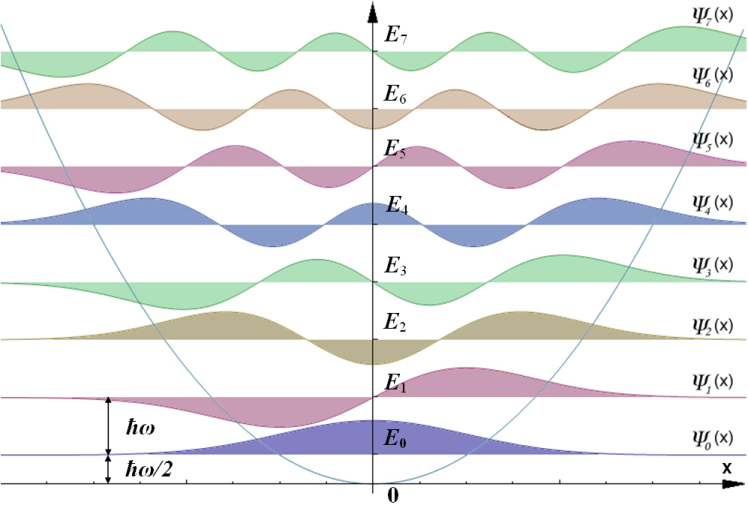
\includegraphics[scale=0.3]{harmonic-oscillator-states.png}
    \end{center}

    \header{General Forms for Solving Free Particle Problems}

    For many potentials, particles appear in \underline{scattered states},
    instead of bound states. In these cases, energies are not quantized
    and general forms are computed over integrals, not sums.
    \gap
    For the case of the \underline{free particle}, where the 
    potential is zero everywhere, one can find the solution using the
    following procedure.
    \begin{enumerate}
        \item Identify $\phi(k)$, which is the distribution of states 
        over the variable $k$, using a Fourier transform:
        \begin{align*}
            \phi(k) = \frac{1}{\sqrt{2\pi}} \int_{-\infty}^{\infty}\Psi(x, 0)e^{-ikx}dx.
        \end{align*}
        \item Transform the function out of the frequency domain using 
        another Fourier transform:
        \begin{align*}
            \Psi(x,t) = \frac{1}{\sqrt{2\pi}}\int_{-\infty}^{\infty} \psi(k) e^{i\left(kx - \frac{\hbar k^2}{2m}t\right)} dk.
        \end{align*}
    \end{enumerate}

    The distribution of states $\phi(k)$ in the general solution is known 
    as the \underline{wavepacket}. There are two velocities that are important
    in this case.
    \begin{itemize}
        \item \sheader{Phase Velocity} $\ds v_\textrm{phase} = \frac{\omega}{k} = \frac{\hbar k}{2m} = \sqrt{\frac{E}{2m}}$
        \item \sheader{Group Velocity} $\ds v_\textrm{group} = 2v_\textrm{phase} = \frac{d\omega}{dk}$
    \end{itemize}
    In all of these forms, $k$ is $k_0$, which is the fundamental 
    frequency of the group.
    \gap

    \header{Probabilities and Expectation Values}
    \sheader{Heisenberg Uncertainty Principle}
    \begin{align*}
        \sigma_x \sigma_p \geq \frac{\hbar}{2}
    \end{align*}

    \header{Orthogonality}

    \begin{itemize}
        \item The stationery states in the infinite square well are orthogonal.
        \item $\ds \int_{0}^{L} \sin \left(\frac{n\pi x}{L}\right) \sin \left(\frac{m\pi x}{L}\right) dx = 0 $
        \item $\ds \int_{0}^{L} \cos \left(\frac{n \pi x}{L}\right) \cos \left(\frac{m \pi x}{L}\right) dx = 0$
        \item $\ds \int_{0}^{L} \sin \left(\frac{n \pi x}{L}\right) \cos \left(\frac{m \pi x}{L}\right) dx = 0$
        \item $\ds \int f_\textrm{even}(x) f_\textrm{odd}(x) dx = 0$
        \item $\ds \int_{0}^{L} \sin \left(\frac{n\pi x}{L}\right) \sin \left(\frac{n\pi x}{L}\right) dx = \frac{L}{2}$
        \item $\ds \int_{0}^{L} \cos \left(\frac{n\pi x}{L}\right) \cos \left(\frac{n\pi x}{L}\right) dx = \frac{L}{2}$
    \end{itemize}

    \header{Probabilites and Such}

    We can define the probability of an event $j$ given the total number of 
    events $N$ and the total number of times it occurs $N(j)$:
    \begin{align*}
        P(j) = \frac{N(j)}{N}.
    \end{align*}
    In discrete variables, if we seek to find the average event $j$, denoted by
    $\langle j \rangle$, we can find it with:
    \begin{align*}
        \langle j \rangle = \frac{\sum j N(j)}{N} = \sum_{j = 0}^\infty j P(j).
    \end{align*}

    The \underline{standard deviation} of an event is important to define:
    \begin{align*}
        \sigma = \sqrt{\langle j^2 \rangle - \langle j \rangle^2}
    \end{align*}

    Similar formulae can also be applied to continuous variables. First, we 
    define the \underline{probability density} of some quantity as $\rho(x) dx$,
    that is $\rho(x)dx$ is the probability that an individual (chosen at random)
    lies between $x$ and $(x + dx)$. Hence, it follows that:
    \begin{align*}
        P_{ab} = \int_a^b \rho(x) dx.
    \end{align*}

    \pagebreak 

    \header{Expected Values}

    As alluded to prior, we can have certain \underline{expected values} for quantities,
    that is, the average value for that quantity over all time. In general, for some quantity $Q$, this is given
    by:
    \begin{align*}
        \langle Q(x, p) \rangle = \int_{-\infty}^{\infty} \Psi^* \left[Q\left(x, -i\hbar \frac{\partial}{\partial x}\right)\right]\Psi dx
    \end{align*}
    Where $Q(x,p)$ is some operator that can be described as a function of $x$ and $p$.
    \gap
    Hence, we can define some common operators:
    \begin{itemize}
        \item \sheader{Position Operator, $x$} $x$.
        \item \sheader{Momentum Operator, $\hat{p}$} $\hat{p} = -i\hbar \frac{\partial}{\partial x}$.
    \end{itemize}
    Energy is another expected value, but obtaining it in bound states is a bit difficult.
    It can be obtained as follows:
    \begin{align*}
        \langle E \rangle = \sum_{n = 1}^\infty |c_n|^2 E_n.
    \end{align*}

    \header{Important Integrals}

    There are some important integrals that often come up:
    \begin{align*}
        \int_{-\infty}^\infty e^{-\frac{x^2}{a^2}}dx = \sqrt{\pi} a && \int_{-\infty}^\infty x^2 e^{-\frac{x^2}{a^2}} dx = \frac{\sqrt{\pi} a^3}{2}
    \end{align*}

\end{document}